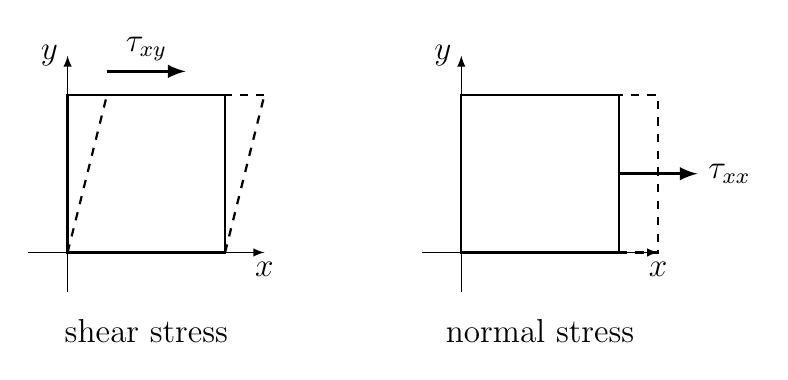
\begin{tikzpicture}[>=latex, scale=1.0, font=\large]
    % Shear and normal stress on a fluid element (revision deck)
    \tikzset{axis/.style={->, thin}, solidline/.style={thick}, dashedline/.style={thick, dashed}, forcearrow/.style={->, very thick}}
    \begin{scope}[shift={(0,0)}]
        \draw[axis] (-0.5,0) -- (2.5,0) node[below] {$x$}; \draw[axis] (0,-0.5) -- (0,2.5) node[left] {$y$};
        \draw[solidline] (0,0) rectangle (2,2);
        \draw[dashedline] (0,0) -- (0.5,2); \draw[dashedline] (2,0) -- (2.5,2); \draw[dashedline] (0.5,2) -- (2.5,2);
        \draw[forcearrow] (0.5, 2.3) -- (1.5, 2.3) node[midway, above] {$\tau_{xy}$};
    \end{scope}
    \begin{scope}[shift={(5,0)}]
        \draw[axis] (-0.5,0) -- (2.5,0) node[below] {$x$}; \draw[axis] (0,-0.5) -- (0,2.5) node[left] {$y$};
        \draw[solidline] (0,0) rectangle (2,2);
        \draw[dashedline] (2,0) -- (2.5,0) -- (2.5,2) -- (2,2);
        \draw[forcearrow] (2, 1.0) -- (3.0, 1.0) node[right] {$\tau_{xx}$};
    \end{scope}
    \node at (1, -1.0) {shear stress}; \node at (6, -1.0) {normal stress};
\end{tikzpicture}
